\chapter{Basic Functions}\label{Basic Functions}


\section{Absolute Value function/ Modulus Function ( $\dabs{x}$ ) \cite{wiki/Absolute-value}}\label{Basic Functions/Absolute Value function or Modulus Function}

\begin{table}[H]
    \begin{minipage}{0.35\linewidth}
        $
            f(x) 
            = \dabs{x}
            = \begin{dcases}
                x   & \text{ if } x \geq 0 \\
                -x  & \text{ if } x < 0
            \end{dcases}
        $
    \end{minipage}
    \begin{minipage}{0.55\linewidth}
        \begin{figure}[H]
            \centering
            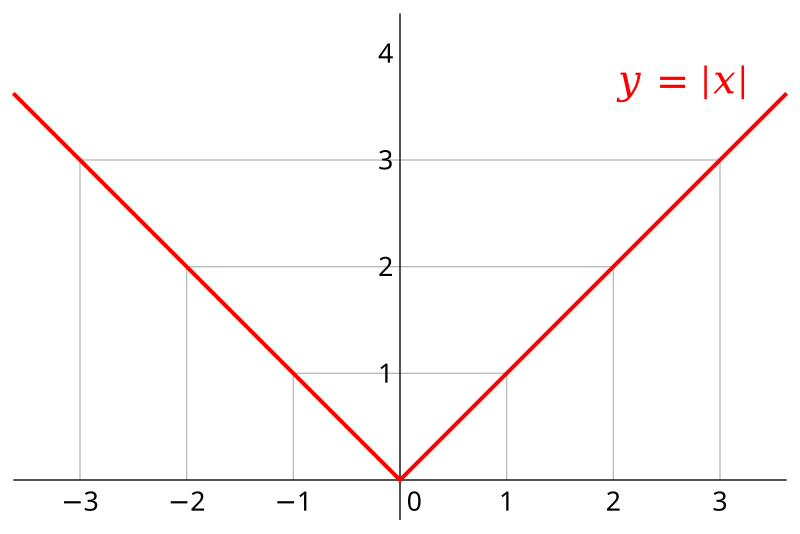
\includegraphics[width=0.5\linewidth, height=5cm, keepaspectratio]{images/basic_math/Absolute_value.svg.png}
            \caption{Absolute Value function/ Modulus Function \cite{wiki/Absolute-value}}
        \end{figure}
    \end{minipage}
\end{table}

\begin{lstlisting}[
    language=Python, 
    caption=Absolute value function
]
def get_absolute_value(val):
    if val >= 0:
        return val
    else:
        return -1 * val
\end{lstlisting}

\subsection*{Properties}

\subsubsection*{Fundamental properties \cite{wiki/Absolute-value}} \label{Basic Functions/Absolute Value function or Modulus Function/Fundamental properties}

\begin{customArrayStretch}{1.2}
\begin{tabular}{r l l}
     1. & ${\displaystyle |a|\geq 0}$ & Non-negativity \\
     
     2. & ${\displaystyle |a|=0\iff a=0}$ & Positive-definiteness \\
     
     3. & ${\displaystyle |ab|=\left|a\right|\left|b\right|}$ & 	Multiplicativity \\
     
     4. & ${\displaystyle |a+b|\leq |a|+|b|}$ & 	Subadditivity, specifically the triangle inequality \\
\end{tabular}
\end{customArrayStretch}

\subsubsection*{Additional useful properties \cite{wiki/Absolute-value}} \label{Basic Functions/Absolute Value function or Modulus Function/Additional useful properties}

\begin{customArrayStretch}{1.5}
\begin{tabular}{r l p{13cm}}
     1. & ${\displaystyle {\bigl |}\left|a\right|{\bigr |}=|a|}$ & 	Idempotence (the absolute value of the absolute value is the absolute value) \\
     
     2. & ${\displaystyle \left|-a\right|=|a|}$ & Evenness (reflection symmetry of the graph) \\
     
     3. & ${\displaystyle |a-b|=0\iff a=b}$ & 	Identity of indiscernibles (equivalent to positive-definiteness) \\
     
     4. & ${\displaystyle |a-b|\leq |a-c|+|c-b|}$ & 	Triangle inequality (equivalent to subadditivity) \\
     
     5. & ${\displaystyle \left|{\frac {a}{b}}\right|={\frac {|a|}{|b|}}\ }$ (if ${\displaystyle b\neq 0}$) & 	Preservation of division (equivalent to multiplicativity) \\
     
     6. & ${\displaystyle |a-b|\geq {\bigl |}\left|a\right|-\left|b\right|{\bigr |}}$ & 	Reverse triangle inequality (equivalent to subadditivity) \\
\end{tabular}
\end{customArrayStretch}

\subsection*{Inequalities} \label{Basic Functions/Absolute Value function or Modulus Function/Inequalities}

\begin{enumerate}
    \item ${\displaystyle |a|\leq b\iff -b\leq a\leq b}$

    \item ${\displaystyle |a|\geq b\iff b\leq a\leq -b\ }$

\end{enumerate}

\subsection*{Derivative} \label{Basic Functions/Absolute Value function or Modulus Function/Derivative}

\begin{enumerate}
    \item $
        {\displaystyle {\frac {d\left|x\right|}{dx}}={\frac {x}{|x|}}={\begin{cases}-1&x<0\\1&x>0\end{cases}}}
    $

    \item $
        {\displaystyle {d \over dx}f(|x|)={x \over |x|}(f'(|x|))}
    $ \hfill (discontinuous at $x=0$)

    \item $
        {\displaystyle {d \over dx}|f(x)|={f(x) \over |f(x)|}f'(x)}
    $ \hfill (discontinuous at $f(x)=0$)
\end{enumerate}


\subsection*{Anti-derivative/ Integral} \label{Basic Functions/Absolute Value function or Modulus Function/Anti-derivative or Integral}

$
    {\displaystyle \dint \left|x\right|dx={\dfrac {x\left|x\right|}{2}}+C}
$



